\section{MindSqualls}
\mindsqualls er et .NET bibliotek til LEGOs NXT robotter.
\mindsqualls tillader kommunikation med NXT enheder via. Bluetooth og USB og fungerer ved at sende og modtager beskeder over disse to teknologier.
Biblioteket er skrevet i \csharp og kan dermed anvendes af alle de .NET kompatible sprog.

I det følgende afsnit gives en kort beskrivelse af bibliotekets struktur samt dets anvendelse.

\subsection{Abstraktion}
For at gøre det nemt at arbejde med NXT motorer og sensorer er der i \mindsqualls lavet en abstraktion over disse.
Hver type I/O er således implementeret i hver sin klasse med passende funktioner.
Figur \ref{mindsqualls:structure} viser et klassediagram, der beskriver relationerne mellem de primære klasser i \mindsqualls biblioteket.

\begin{figure}
\centering
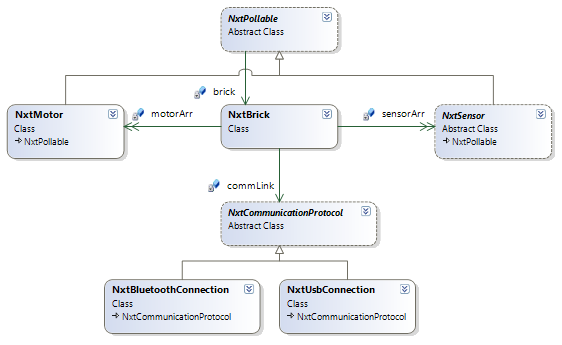
\includegraphics[width=0.8\textwidth]{mindsqualls}
\caption{Den overordnede \mindsqualls struktur}
\label{mindsqualls:structure}
\end{figure}

\subsection{Forbindelse til NXT}
\mindsqualls opretter forbindelse til NXT enheden vha. klassen \lstinline[style=csharp]!NxtCommunicationProtocol!.
Klassen fungerer, som navnet indikerer, som en protokol ved at definere en række abstrakte funktioner;
Der kan oprettes forbindelse til NXT enheden.
Denne kan afbrydes igen, og det kan til enhver tid fastslås om der er forbindelse til enheden.
Selve kommunikationen sker via kald til funktionen \lstinline[style=csharp]!Send! der tager et array af bytes som input og giver et array af bytes som output.
Altså kan funktionen både sende og modtage beskeder til og fra enheden.
Ved at lave specialiseringer af \lstinline[style=csharp]!NxtCommunicationProtocol! klassen, der definere disse funktioner, kan der kommunikeres med NXT enheden.
Der findes i \mindsqualls to specialiseringer af protokollen;
\begin{itemize}
\item \lstinline[style=csharp]!NxtUsbConnection!\\
Tillader kommunikation via USB (kablet)
\item \lstinline[style=csharp]!NxtBluetoothConnection!\\
Tillader kommunikation via Bluetooth (trådløst)
\end{itemize}

